\maketitle

\begin{abstract}
In the life-cycle of objects there are different phases. The phase in which an object currently is, affects how it is handled in an application; however phase shifts are often implicit. Selecting objects according to such phase shifts results in scattered and tangled code. In this study we propose a new kind of pointcut, called \emph{instance pointcuts}, for creating and maintaining sets of objects according to events in their life-cycle; these events are selected with pointcut-like specifications. Instance pointcuts can be reused, by refining their selection criteria, e.g., by restricting the scope of an existing instance pointcut; and they can be composed, e.g., by set operations. These features make instance pointcuts easy to evolve according to new requirements. Our approach improves modularity by providing a fine-grained mechanism and a declarative syntax to create and maintain phase-specific object sets.
\end{abstract}

% A category with the (minimum) three required fields
\category{D.3.1}{Formal Definition and Theory}[syntax, semantics]
%A category including the fourth, optional field follows...
\category{D.3.4}{Processors}[code generation]

\section{Introduction}
In object-oriented programming (OOP), objects encapsulate state and behaviour; objects also have a life-cycle, which means that the same object can play different roles at different times.
Which role an object is currently playing can affect the object's own behaviour or how it is handled.
Often the shift from one life-cycle phase to another is implicitly marked by events, e.g., passing an object from one client to another.

As an example of relevant phases in the life-cycle of objects, consider an online store application with ``vendor'' objects representing the suppliers and ``product'' objects representing the products they sell. 
Assume we would like to keep the list of products which were applied the happy-hour discount. For each product, a different time slot can be defined as the happy hour, so the list of products that are discounted is changing over time. Grouping objects according to criteria which cannot be directly accessed through programming language constructs --- such as which class they were initialized in, which method they were passed to as an argument, or (as in the example) the time at which they are passed to a method, requires invasive insertion of bookkeeping code.

Aspect-oriented programming (AOP) can be applied to separate this bookkeeping code from the business logic of the program. But in AOP, \emph{pointcuts} select sets of so-called \emph{join points} which are points in time during the execution of the program. Current aspect-oriented languages do not support a \emph{declarative specification} of the objects belonging to a life-cycle phase; instead an \emph{imperative implementation}, typically following the same pattern, is required for collecting those objects.

A consequence of such an imperative solution is reduced readability and maintainability due to scattering, tangling and boilerplate code. Another issue is the lack of composition and checking mechanisms for the imperative bookkeeping. It is not possible to reuse the previously written code which results in code that is hard to maintain and hinders software evolution. Also the warnings and errors do not indicate the proper context and relevant information to guide the programmer.


To offer better support for processing objects according to their life-cycle phases, we propose a new mechanism, called \emph{instance pointcuts}, to select sets of objects based on the events in their execution history.
Instance pointcuts are used to declare the beginning and the end of a life-cycle as events. Instance pointcuts can be reused via refinement and composition operations and their implementation provides checks to aid correctness. 

An instance pointcut's concise definition consists of three parts: an identifier, a type which is the upper bound for all the selected objects in the phase-specific set, and a specification of relevant objects.
For a basic instance pointcut definition, the specification utilizes \emph{pointcut expressions} to select events that define the start and the end of life-cycle phases and to expose an object. At these events, the object is added or removed from the set maintained by the instance pointcut. 
New instance pointcuts can be derived from existing ones. Firstly, a new instance pointcut can be derived from another one by restricting the type of selected objects. 
Secondly, a new instance pointcut can be created by reusing the object selection expressions of the existing ones.
Lastly, instance pointcuts can be composed arbitrarily by means of set operators. 

In this paper we present a prototype of instance pointcuts as an extension to AspectJ \cite{kiczales2001overview} and explain its semantics by explaining our compiler which transforms instance pointcuts to plain AspectJ and advanced dispatching library calls. 

The declarative nature of instance pointcuts give rise several compile-time checks which are not automatically possible with equivalent imperative code. 
Such checks are important to notify the developer when the instance pointcut set is guaranteed to be empty, incompatible types are used  in compositions and refinements, etc.  These checks help the developer to implement his concern correctly and achieve consistence in phase-specific object sets. 


The rest of the paper is organized as follows, in section~\ref{sect:motivation} we present a small case study and explain our motivation for the proposed approach. In section~\ref{sect:approach}, a detailed description of instance pointcuts and its various features are presented. Section~\ref{sect:compilation} explains how instance pointcuts are compiled. We then present a discussion on the validation of our approach and outline possible checks in section~\ref{sect:checking}. We conclude by discussing related work and giving a summary of our approach.


\section{Motivation}
\label{sect:motivation}
Supporting \emph{unanticipated} extensions introduces new implementation concerns like creating specific object sets.
Objects can be grouped according to how they are used (passed as arguments to method calls, act as receiver or sender for method calls, etc.) and concerns of an application may be applicable only to objects used in a specific way.
Therefore we must be able to identify and select such objects.
We want to expose sets of objects belonging to the same life-cycle phase by means of a dedicated language construct such that the implementation of phase-dependent concerns can be explicit.

\begin{figure*}
\centering
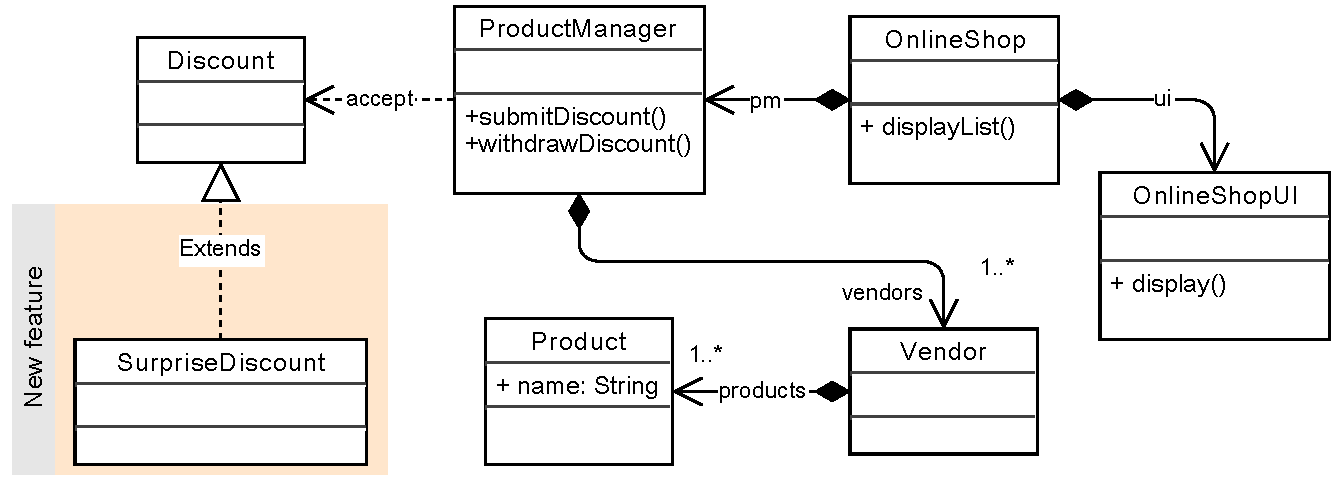
\includegraphics[width=0.75\textwidth]{images/aosd2013onlineshop.pdf}%
\vspace{10pt}
\caption{Part of an online shop application}%
\label{fig:shop}%
\end{figure*}

In Figure~\ref{fig:shop}, we outline a part of the architecture of an online shop application. We use this scenario to give examples of grouping objects into sets according to how they are used and how to use these sets in the implementation of concerns. 
%At the end of this section, we conclude requirements for solving the encountered challenges in these examples.

\subsection{Example Architecture}
In an online shop application, objects of the same type can exist at different stages of their life-cycle. In Figure~\ref{fig:shop} the static structure of a simplified online shop is shown. This structure shows part of the system from the \lstinln{Vendor} and the \lstinln{OnlineShop}'s perspective. \lstinln{Vendor}s can submit different kinds of \lstinln{Discount}s (not shown in the figure) to the \lstinln{ProductManager} for the \lstinln{Product}s they are selling. \lstinln{Product} is the root of the type hierarchy that represents different kinds of items that is sold in the online shop and is parent to the classes such as \lstinln{BeautyProduct}, \lstinln{SportProduct} (not shown in the figure). Each \lstinln{Product} holds a list of \lstinln{Discount}s they are applied. The \lstinln{OnlineShop} has a user interface represented by the \lstinln{OnlineShopUI} class, which is used to display information to the customers. 


\subsection{Unanticipated Extensions}
A new feature is added to the online shop which requires creating an alert when a product is applied a surprise discount. The list of surprise discounted products should be available to the user at any time. The surprise discounts are submitted by \lstinln{Vendor}s and they can be submitted or withdrawn any time.  In order to realize this extension in an OO-approach, we need to change several classes to host this extension. First the class \lstinln{ProductManager} should keep a set of \lstinln{Product}s which are applied a surprise discount, in listing~\ref{lst:discountalert} this is shown in line~\ref{surpdisset}. This set is updated when a new discount of type \lstinln{SurpriseDiscount} is submitted or withdrawn (lines~\ref{surpset:begin}--~\ref{surpset:end}). There should also be some changes in the \lstinln{OnlineShop} class. A \lstinln{createDiscountAlert} method should be added. Also the \lstinln{displayList} method should be updated to include the \lstinln{surpriseDiscount} list defined in the \lstinln{ProductManager} class.


\begin{lstlisting}[float, caption={A Java implementation of discount alert concern}, label={lst:discountalert}]
class ProductManager{
	...
	Set<Product> surpriseDiscount = createSet(); ~\label{surpdisset}~
	public void submitDiscount(Product p, Discount d){~\label{surpset:begin}~
		...
		if(d instanceof SurpriseDiscount){
			surpriseDiscount.add(p);
			OnlineShop.createDiscountAlert(p);
		}
	}
	public boolean withdrawDiscount(Product p, Discount d){
		...
		if(d instanceof SurpriseDiscount)
			surpriseDiscount.remove(p);
	}~\label{surpset:end}~
}
class OnlineShop{//SINGLETON
	...
	public void createDiscountAlert(Product p){
		//create surprise discount alert for p
	}
	public void displayList(String listType){
		if(listType.equals(``surprise'')
			INSTANCE.getUI().display(ProductManager.surpriseDiscount);
	}
}
\end{lstlisting}


 OO-solution is scattered among the classes \lstinln{ProductManager} and \lstinln{OnlineShop} and tangled with multiple methods.

An aspect-oriented implementation can offer a better solution by encapsulating the concern in an aspect. Listing~\ref{lst:discountaop} shows a possible solution. The set of products which are applied a surprise discount is kept in the aspect (line~\ref{daop:set}). The following two pointcuts \lstinln{submit} and \lstinln{withdraw} selects the products to which a \lstinln{SurpriseDiscount} is applied (lines~\ref{daop:pc:submit}~\textendash~\ref{daop:pc:wdraw}). The corresponding advice declarations for these pointcuts maintain the \lstinln{surpriseDiscount} set. The \lstinln{submit} pointcut triggers the surprise discount alert method (line~\ref{daop:alert}). There is also the \lstinln{display} pointcut (line~\ref{daop:pc:display}), which intercepts the call to \lstinln{displayList} method and add the condition for the surprise discount list in an around advice (lines~\ref{daop:around:begin}~\textendash~\ref{daop:around:end}). This aspect includes an inter-type declaration which adds the \lstinln{createDiscountAlert} method to the \lstinln{OnlineShop} class.


\begin{lstlisting}[float=h, caption={An AspectJ implementation of discount alert concern}, label={lst:discountaop}]
aspect SDiscount{
	Set<Item> surpriseDiscount = createSet();~\label{daop:set}~
	pointcut submit(Product p): call(* ProductManager.submitDiscount(..)) && args(p, SurpriseDiscount); ~\label{daop:pc:submit}~
	pointcut withdraw(Product p): call(* ProductManager.withdrawDiscount(..)) && args(p, SurpriseDiscount); ~\label{daop:pc:wdraw}~
	pointcut display(String listType): call(* OnlineShop.displayList(..)) && args(listType);~\label{daop:pc:display}~
	after(Product p): submit(p){
		surpriseDiscount.add(p);
		OnlineShop.INSTANCE().createDiscountAlert(p);~\label{daop:alert}~
	}
	after(Product p):withdraw(p){
		if(surpriseDiscount.contains(p))
			supriseDiscount.remove(p);}
	}
	void around(String listType):display(listType){~\label{daop:around:begin}~
		if(listType.equals(``surprise'')
			OnlineShop.instance().getUI().display(surpriseDiscount);
		proceed(listType);	
	} ~\label{daop:around:end}~
	public void OnlineShop.createDiscountAlert(Product p){
		//create surprise discount alert for a product
	}
}
\end{lstlisting}

\subsection{Problem Statement}

AOP already helps to localize the concern and to add it without the need to modify existing code.
%But most of the implementation of the surprise discount concern as shown in Listing~\ref{lst:discountaop} consists of boilerplate code .
However maintenance of the \lstinln{surpriseDiscount} set requires the same boilerplate code as the OO solution does.
Essentially the code selects \lstinln{Product} objects based on the discount they are applied to and deselect them once they are rid of this discount. 
This marks a phase in the life-cycle of a \lstinln{Product} object None of the solutions presented in this section offer declarative means to define such a life-cycle phase.
Furthermore, reusing such existing reifications of objects in a specific life-cycle phase  by refining or composing them is not conveniently supported at all; e.g., if we want to find the subset of \lstinln{BeautyProduct}s of the \lstinln{surpriseDiscount} set, we have to iterate over it and check instance types to create a new set. Such imperative definitions are difficult or impossible to analyze by the compiler. Checks like determining if the set is empty cannot be performed. From this motivating example we conclude our problem statement as follows.

Creating object sets according to execution events is a cross-cutting concern. Current programming approaches only provide imperative ways to maintain special kinds of object sets which result in code that is marginally concern-specific and mostly boilerplate, which is scattered and tangled. There are no built-in mechanisms for composing such sets. The maintenance costs of such programs hinder software evolution and their imperative nature prevents useful checks.


